, а так же переопределена виртуальная функция \textbf{run()} запускающая
поток с задачей.

Внутри этого потока создается TCP сокет и происходит попытка открыть TCP
соединение, если спустя 500 мс соединение не было установлено, то порт
считается закрытым и задача завершает с кодом 1, иначе при установленном
соединении сокет закрывает соединение и задача завершается с кодом 0.

\hypertarget{ux440ux443ux43aux43eux432ux43eux434ux441ux442ux432ux43e-ux43fux43eux43bux44cux437ux43eux432ux430ux442ux435ux43bux44f}{%
\section{Руководство
пользователя}\label{ux440ux443ux43aux43eux432ux43eux434ux441ux442ux432ux43e-ux43fux43eux43bux44cux437ux43eux432ux430ux442ux435ux43bux44f}}

При запуске сканера выводится предупреждение о запрете сканирования в
глобальных сетях.

В поле адрес необходимо ввести сканируемый адрес сети в формате IPv4/

Далее необходимо нажать кнопку ``Сканировать'' для начала процесса
сканирования.

Программа сканирует порты из списка общеизвестных портов
(\textbf{0-1023}) и зарегистрированных портов (\textbf{1024-49151}).

В процессе работы сканера появится шкала прогресса и в логе отобразится
сообщение о старте сканирования.

После завершения работы в логе сканера отобразится список открытых
портов вышеуказанного адреса.

\hypertarget{ux442ux435ux441ux442ux438ux440ux43eux432ux430ux43dux438ux435}{%
\section{Тестирование}\label{ux442ux435ux441ux442ux438ux440ux43eux432ux430ux43dux438ux435}}

\hypertarget{ux438ux441ux445ux43eux434ux43dux44bux435-ux434ux430ux43dux43dux44bux435}{%
\subsection{Исходные
данные}\label{ux438ux441ux445ux43eux434ux43dux44bux435-ux434ux430ux43dux43dux44bux435}}

Для проверки работоспособности программы было совершено сканирование 3
хостов в локальной сети.

\begin{itemize}
\item
  Маршрутизатор.
\item
  ПК, на котором был запущен сканер.
\item
  Смартфон, подключенный к маршрутизатору.
\end{itemize}

\hypertarget{ux442ux435ux441ux442-1.-ux43cux430ux440ux448ux440ux443ux442ux438ux437ux430ux442ux43eux440}{%
\subsection{Тест 1.
Маршрутизатор}\label{ux442ux435ux441ux442-1.-ux43cux430ux440ux448ux440ux443ux442ux438ux437ux430ux442ux43eux440}}

Маршрутизатор с ОС Open-Wrt с вручную открытым портом для SSH (20).

\begin{figure}
\centering
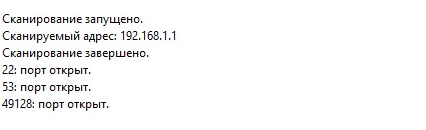
\includegraphics{./files/screenshot2.png}
\caption{Результат работы программы}
\end{figure}

Программа показала что роутере открыты порты:

\begin{itemize}
\item
  22 - порт SSH
\item
  53 - DNS порт
\item
  1009 - неиспользуемый порт
\end{itemize}

\hypertarget{ux442ux435ux441ux442-2.-ux43fux43a}{%
\subsection{Тест 2. ПК}\label{ux442ux435ux441ux442-2.-ux43fux43a}}

Компьютер работает под управление ОС Windows.

\begin{figure}
\centering
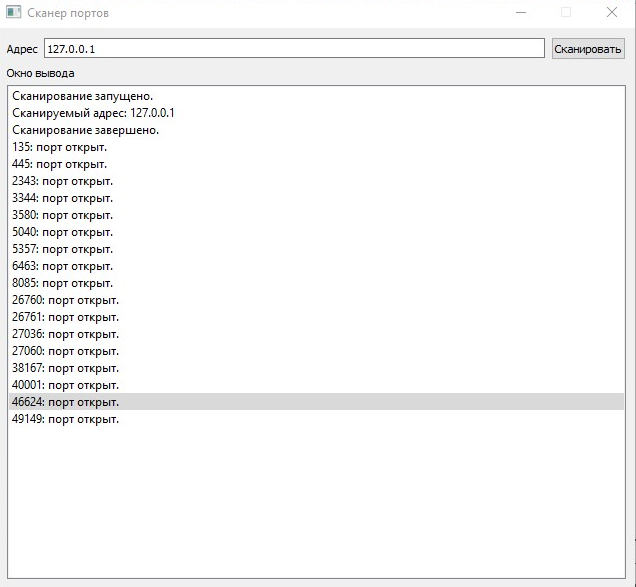
\includegraphics{./files/screenshot.png}
\caption{Результат работы программы}
\end{figure}

Программа показала что на компьютере открыты порты:

\begin{itemize}
\item
  135 - порт EPMAP, Microsoft RPC, Locator service
\item
  445 - порт MICROSOFT-DS
\item
  2343, 3344, 3580, 5040, 5357, 6463, 8085, 26760, 26761, 27036, 27060,
  38167, 40001, 46624, 49139 - неиспользуемые открытые порты.
\end{itemize}

\hypertarget{ux442ux435ux441ux442-3.-ux441ux43cux430ux440ux442ux444ux43eux43d}{%
\subsection{Тест 3.
Смартфон}\label{ux442ux435ux441ux442-3.-ux441ux43cux430ux440ux442ux444ux43eux43d}}

Смартфон под управлением ОС Android с отключенным ABD на порту 5555.

\begin{figure}
\centering
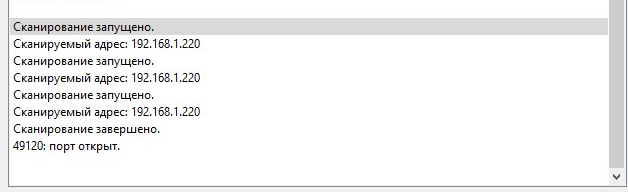
\includegraphics{./files/screenshot3.png}
\caption{Результат работы программы}
\end{figure}

Программа показала что на смартфоне открыты порты:

\begin{itemize}
\tightlist
\item
  1009 - неиспользуемый порт
\end{itemize}

Через 20 секунд после работы сканера, маршрутизатор отключил ПК с
сканером от локальной сети. Сработало правило сетевого экрана.

\hypertarget{ux437ux430ux43aux43bux44eux447ux435ux43dux438ux435}{%
\section{Заключение}\label{ux437ux430ux43aux43bux44eux447ux435ux43dux438ux435}}

В ходе выполнения данной курсовой работы был реализован многопоточный
сканер портов с графическим интерфейсом, а так же проверена его
работоспособность в локальной сети. В процессе написания работы были
изучены различные типы сканирования портов, законность выполнения
сканирования портов, основные диапазоны портов. В ходе написания
программы были изучены принципы построения графических интерфейсов в
библиотеке Qt, а так же архитектурные решения предоставляемые этой
библиотекой для создания многопоточных приложений. При написании сканера
оптимизации для многопоточной работы было применено архитектурный шаблон
``пул'' потоков, из-за технических особенностей ОС Windows был
реализован только 1 тип сканирования портов - TCP, для реализации других
типов сканирования необходимо использовать специализированные драйвера
сетевых устройств, позволяющие работать на уровне IP пакетов.
